\documentclass[12pt, a4paper]{ctexart}
\usepackage[backend=bibtex,citestyle=numeric]{biblatex}
\usepackage{amsmath, amsthm, amssymb, appendix}
\usepackage{bm, fancyhdr, graphicx, mathrsfs, zhnumber}
\usepackage{url}
\usepackage{subfigure}
\usepackage[top=0.5cm, bottom=0.5cm, left=2cm, right=2cm]{geometry}
\usepackage{multirow}
\usepackage{algorithm}
\usepackage{algpseudocode}
\usepackage{amsmath}
\usepackage{algorithmicx}
\usepackage{algpseudocode}
\usepackage{listings}
\usepackage[explicit]{titlesec}
 
\titlespacing*{\section}{0pt}{1.2ex plus .0ex minus .0ex}{.3ex plus .0ex}
\titlespacing*{\subsection}{0pt}{1.2ex plus .0ex minus .0ex}{.3ex plus .0ex}
\geometry{left=2.54cm, right=2.54cm, top=2cm, bottom=2cm}
\linespread{1.25}
\title{Lab2 实验报告}
\author{2100012983 刘逸兴}

\begin{document}
\maketitle
\section{Loop Mesh Subdivision}
算法大致流程:

\begin{enumerate}
    \item 遍历每条边,在每条边上添加新顶点。如果边是边界,则新顶点坐标为两端点坐标平均值。否则如图设置坐标。
    \item 对于每个旧顶点,如图设置坐标。
    \item 按照顺序更新Indices数组,维护Mesh结构。
    \item 重复上述步骤直到达到迭代次数
\end{enumerate}

\begin{figure}[H]
    \centering
    \subfigure[new vertices]{
        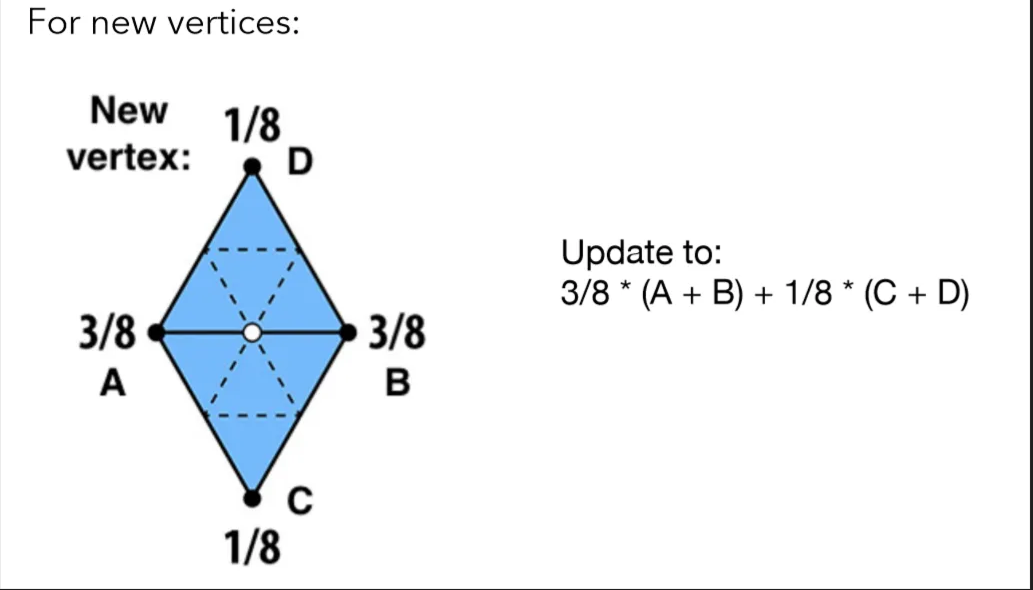
\includegraphics[scale=0.3]{loop0.png}
        }
    \hspace{0.5in}
    \subfigure[old vertices]{
        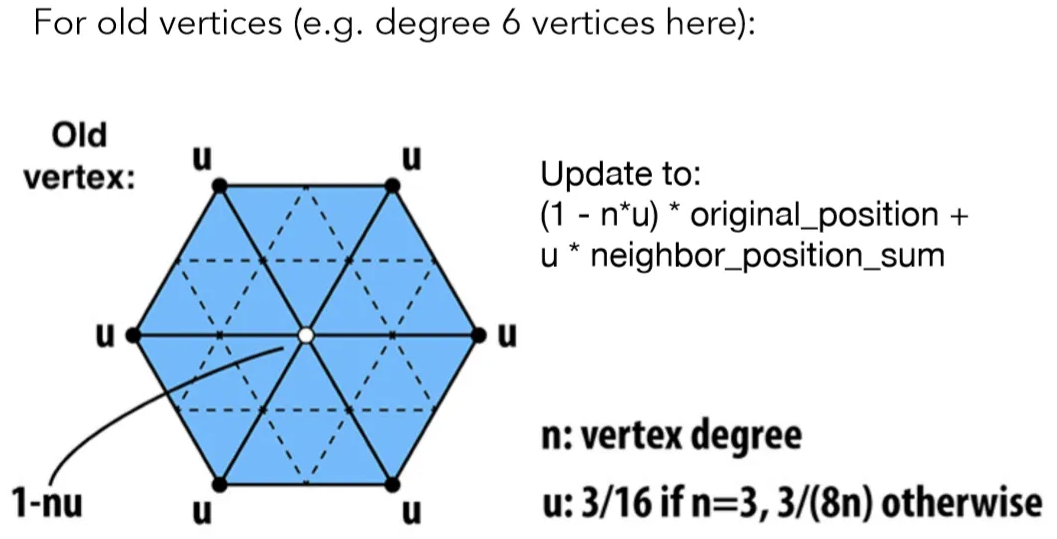
\includegraphics[scale=0.3]{loop1.png}
        }
    \caption{Loop Subdivision}
\end{figure}

得到结果如图:
\begin{figure}[H]
    \centering
    \subfigure[cube, numIteration = 0]{
        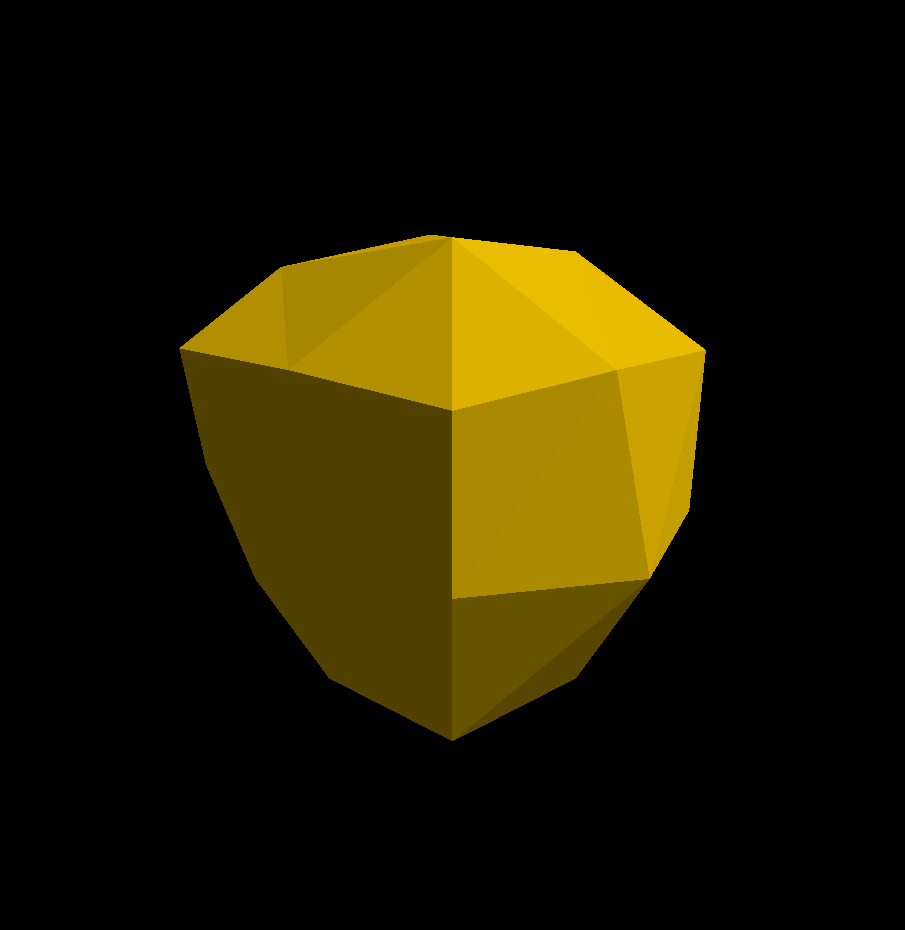
\includegraphics[width=0.3\linewidth]{subdivision_cube_0.png}
        }
    \hspace{0.5in} % 两图片之间的距离
    \subfigure[cube, numIteration = 3]{
      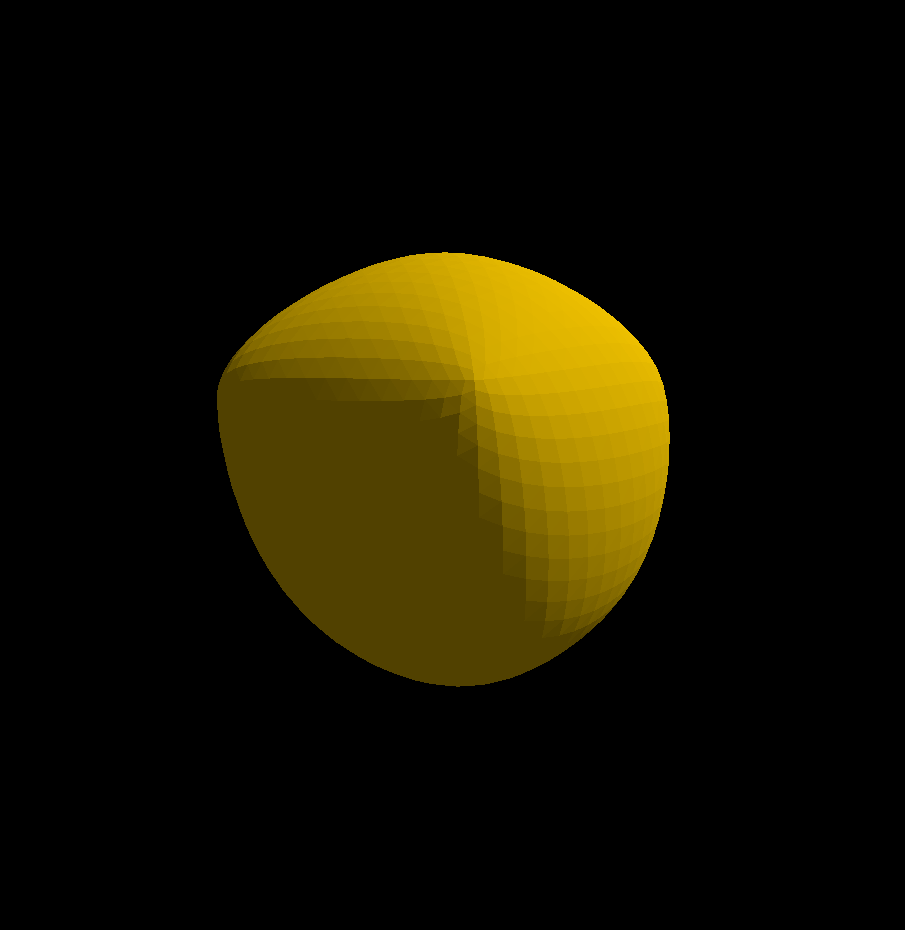
\includegraphics[width=0.3\linewidth]{subdivision_cube_3.png}
      }
    \hspace{0.5in} % 两图片之间的距离
    \subfigure[dinosaur, numIteration = 0]{
        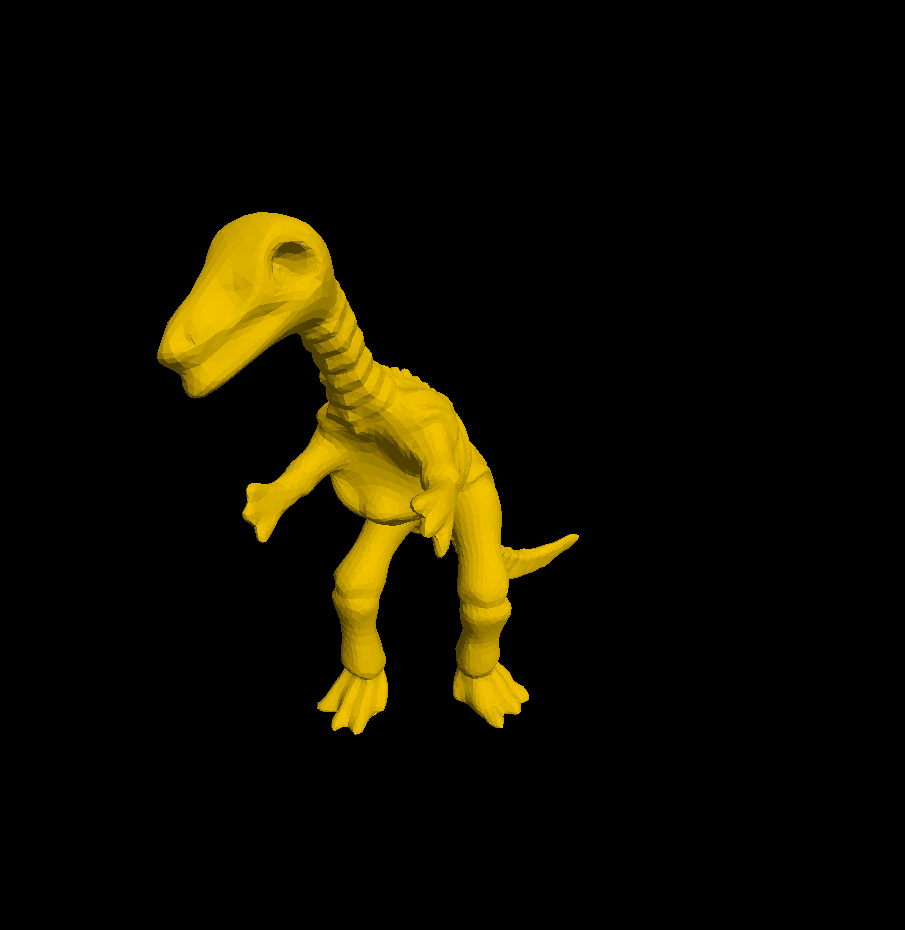
\includegraphics[width=0.3\linewidth]{subdivision_dinosaur_0.png}
        }
    \hspace{0.5in} % 两图片之间的距离
    \subfigure[dinosaur, numIteration = 3]{
    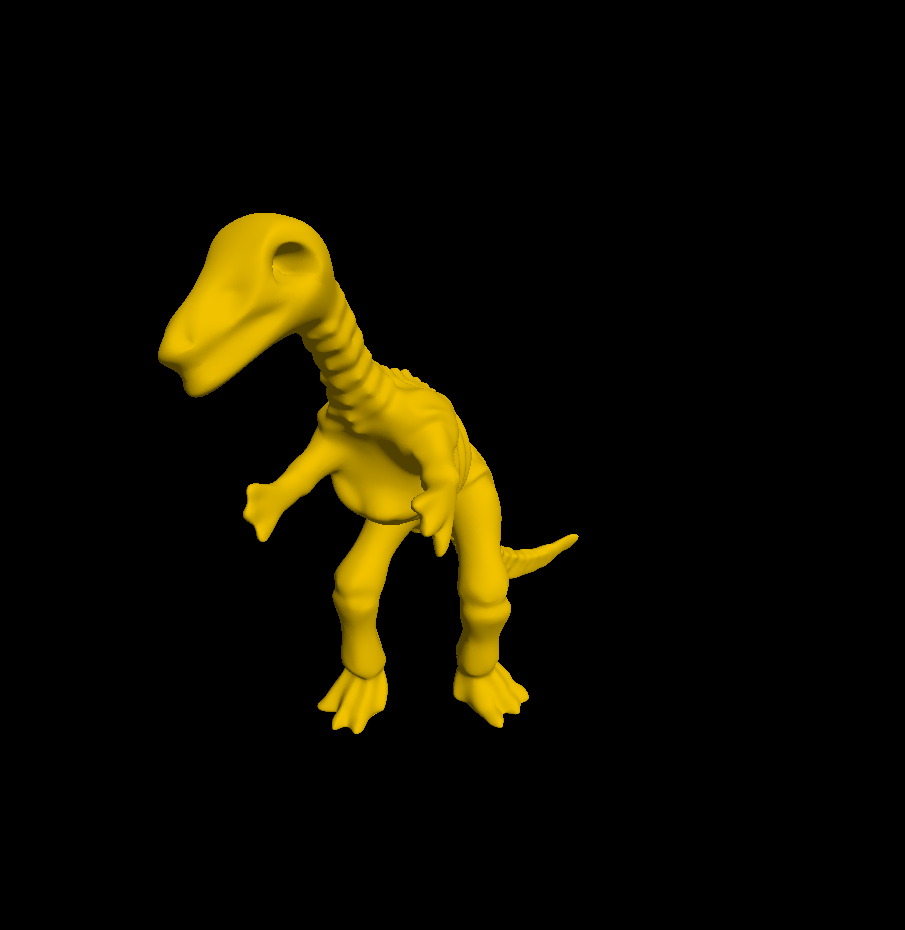
\includegraphics[width=0.3\linewidth]{subdivision_dinosaur_3.png}
      }
    \caption{Mesh Subdivision}
  \end{figure}

\section{Spring-Mass Mesh Parameterization}

算法大致流程:

\begin{enumerate}
    \item 初始化边界点上的uv坐标,这里我用的是圆边界。对于边界点$p(x,y,z)$,初始化坐标为$u = \frac{1}{2} + \frac{x}{2\sqrt{x^{2} + y^{2}}},v=u = \frac{1}{2} + \frac{y}{2\sqrt{x^{2} + y^{2}}}$
    \item 新建数组,存储所有的内部点。
    \item 按照论文中的方法设置$\vec{b},b_{i} = (\sum_{\mbox{j与i相连且j是边界点}} \lambda_{ij} u_{j}, \sum_{\mbox{j与i相连且j是边界点}} \lambda_{ij} v_{j}),\mbox{i是内部点}$
    \item 迭代初值均设为$(0,0)$
    \item 利用Jacobi迭代求解,其中系数矩阵同样按照论文中的方法设置。
\end{enumerate}

为了方便起见,设$\lambda_{ij}$为i的邻居点的个数的倒数。

得到结果如图:
\begin{figure}[H]
    \centering
    \subfigure[numIteration = 0]{
        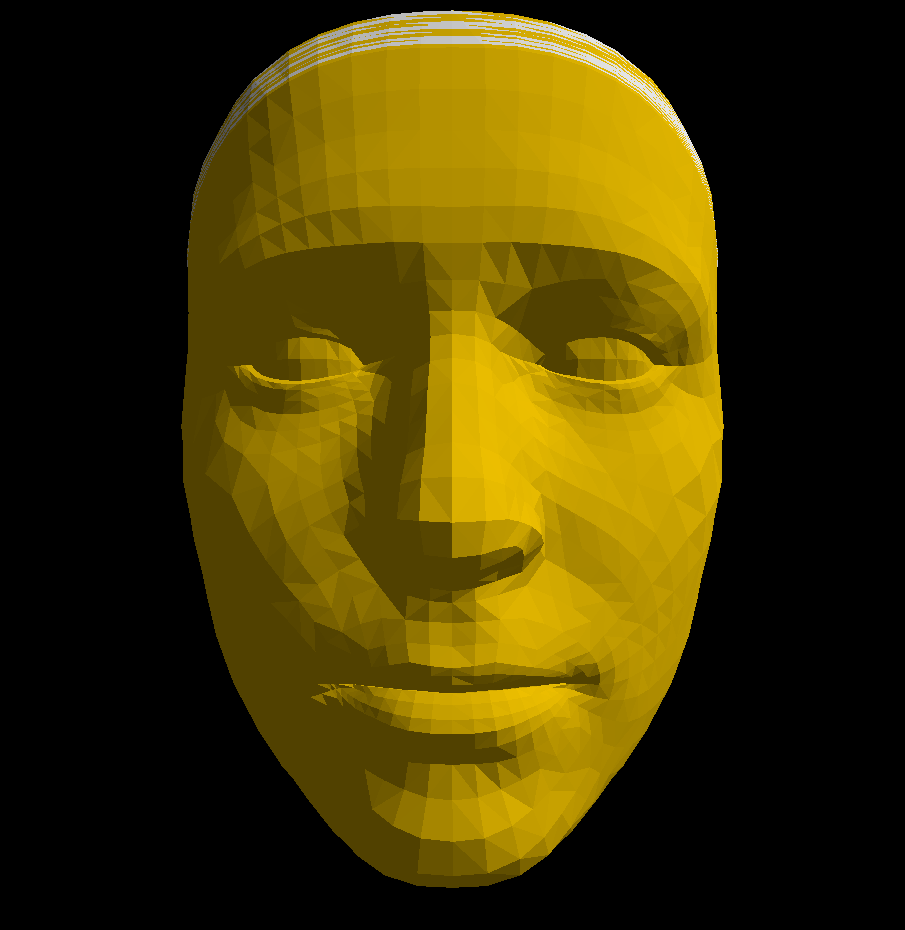
\includegraphics[width=0.3\linewidth]{parameterization.png}
        }
    \hspace{0.5in} % 两图片之间的距离
    \subfigure[numIteration = 25]{
      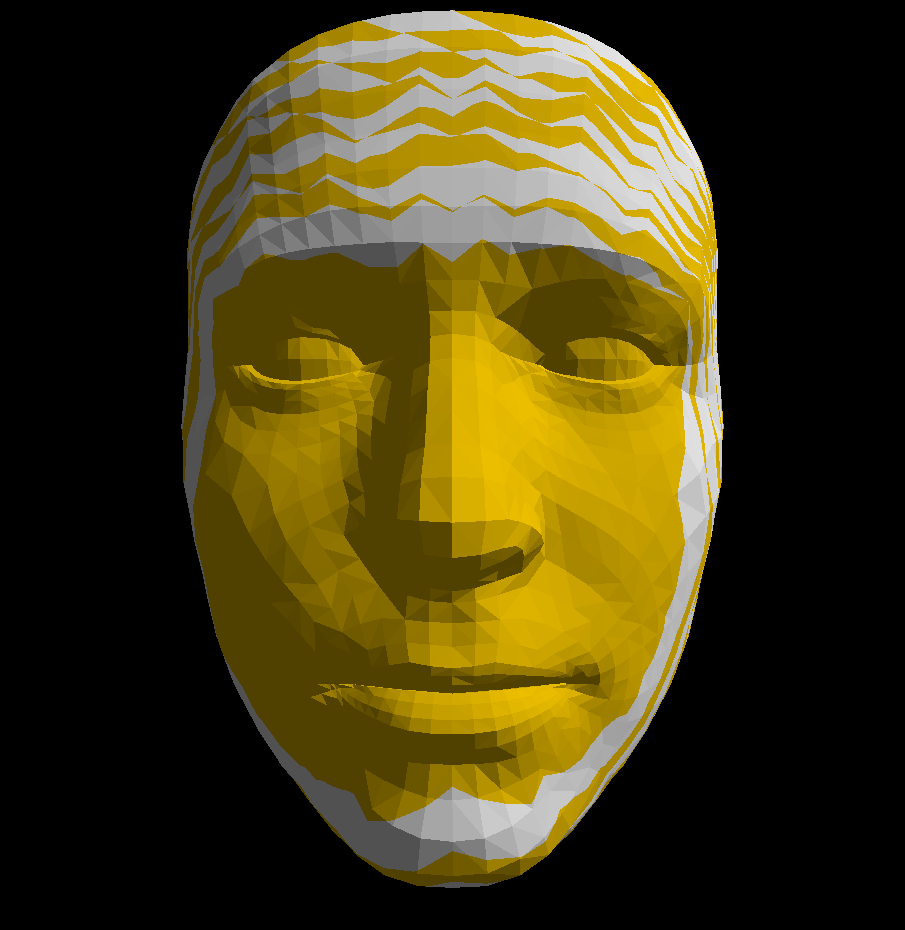
\includegraphics[width=0.3\linewidth]{parameterization_25.png}
      }
    \hspace{0.5in} % 两图片之间的距离
    \subfigure[numIteration = 100]{
        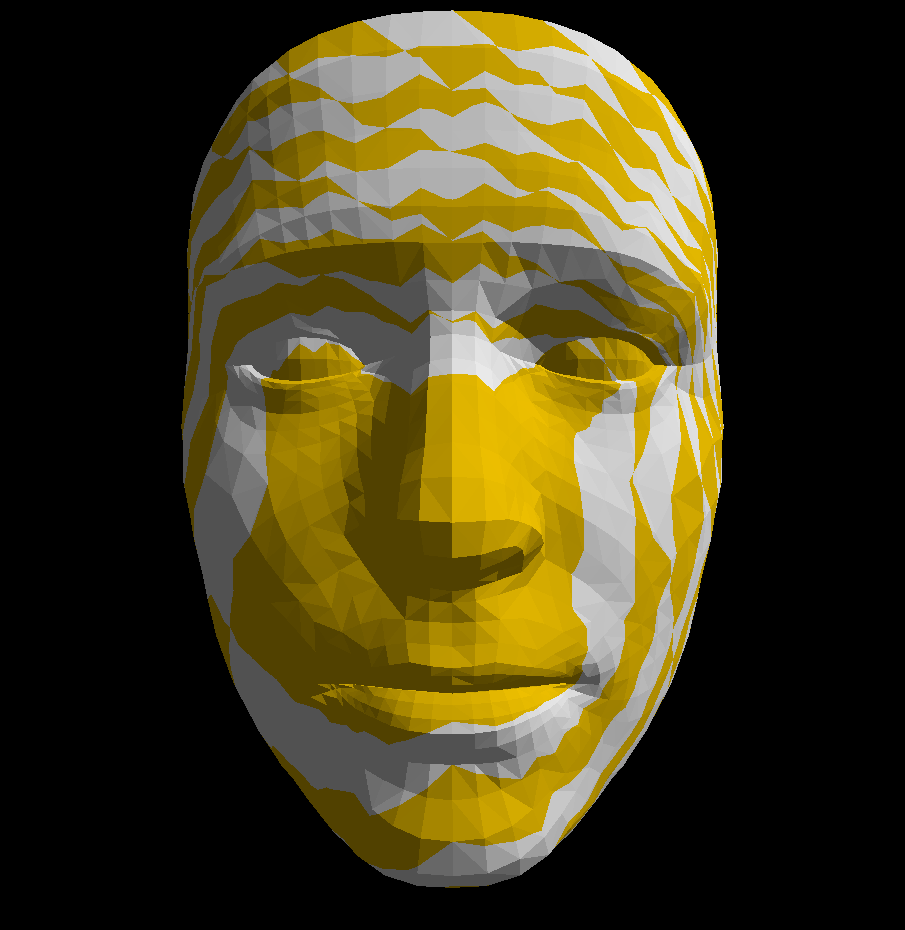
\includegraphics[width=0.3\linewidth]{parameterization_100.png}
        }
    \hspace{0.5in} % 两图片之间的距离
    \subfigure[numIteration = 400]{
    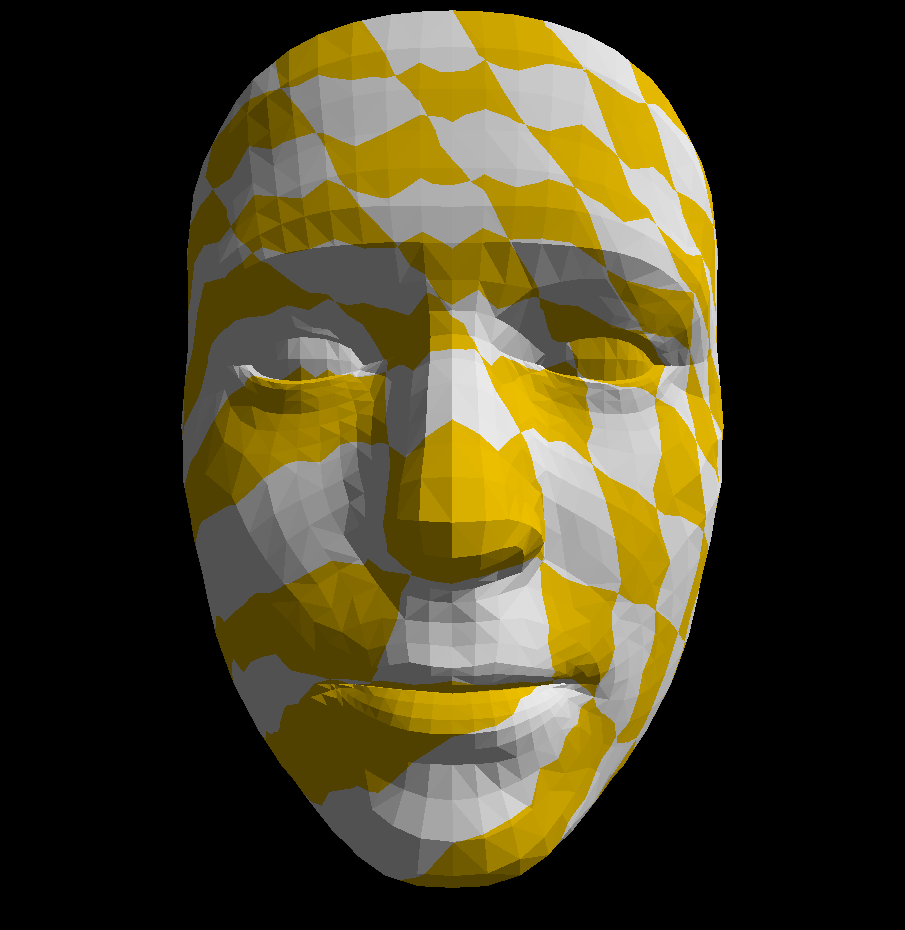
\includegraphics[width=0.3\linewidth]{parameterization_400.png}
      }
    \hspace{0.5in} % 两图片之间的距离
    \subfigure[numIteration = 1000]{
        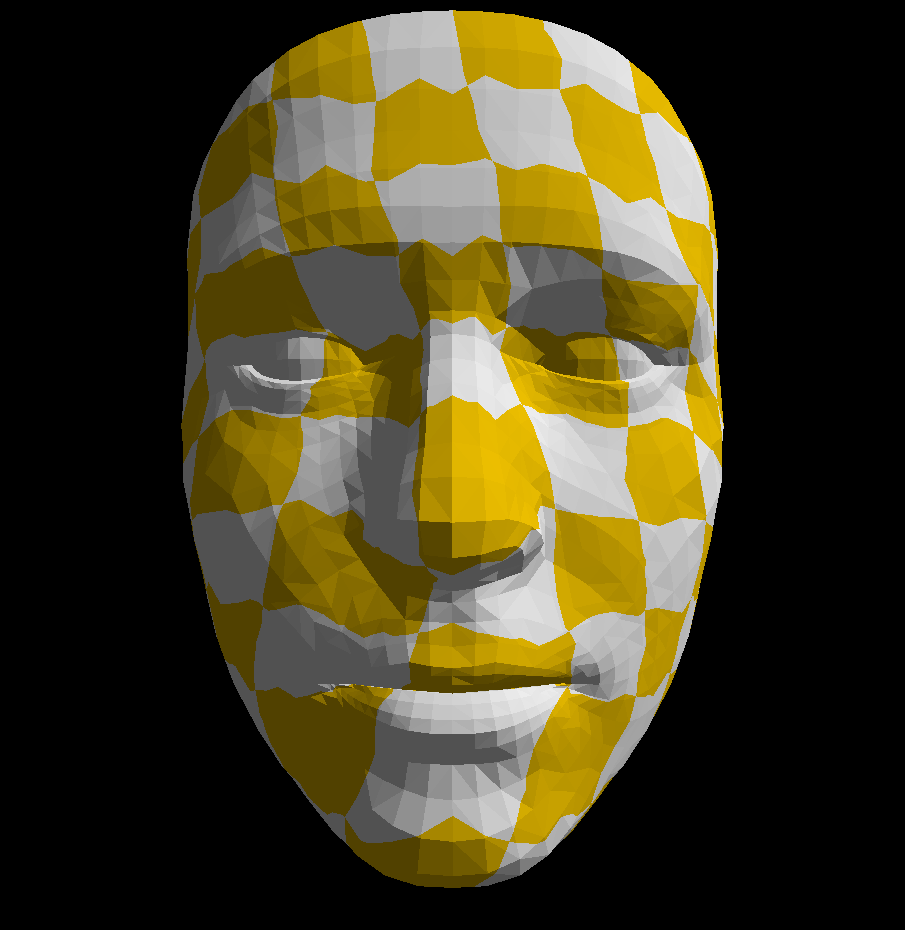
\includegraphics[width=0.3\linewidth]{parameterization_1000.png}
        }
    \caption{Mesh Parameterization}
    % \label{fig:twopicture} 
  \end{figure}

\section{Mesh Simplification}
算法大致流程:

\begin{enumerate}
    \item 对于每个顶点,按照论文中的方法计算其Q矩阵 $Q_{i} = \sum_{p \in planes(v_{i})} (\textbf{p} ^T \textbf{v}) ^2 $
    \item 选取所有合法点对:相邻顶点或者距离小于阈值的点对
    \item 按照论文中的方法计算每对点对的最佳替代点$\bar{v}$,以及损失$cost = \bar{v} ^T (Q_{1}+Q_{2})\bar{v}$
    \item 选择$cost$值最小的点对进行替换,同时更新output中的各个数组以及存储Q矩阵和最佳点对的数组。
    \item 不断重复第四步,直到满足迭代终止条件。
\end{enumerate}

由于没有使用堆结构来维护所有合法点对中$cost$最小的点对,因此该算法时间复杂度较大,同时在第四步更新各个数组的过程中,也没有采取特殊的数据结构,
因而常数也较大。因此对于简化比例较小的情况,只挑选了节点数较小的恐龙图来展示最终的结果。当然,由于恐龙图的拓扑结构较为复杂,这一结果也具有较大的意义。

\begin{figure}[H]
  \centering
  \subfigure[sphere,simplification ratio = 0.8]{
      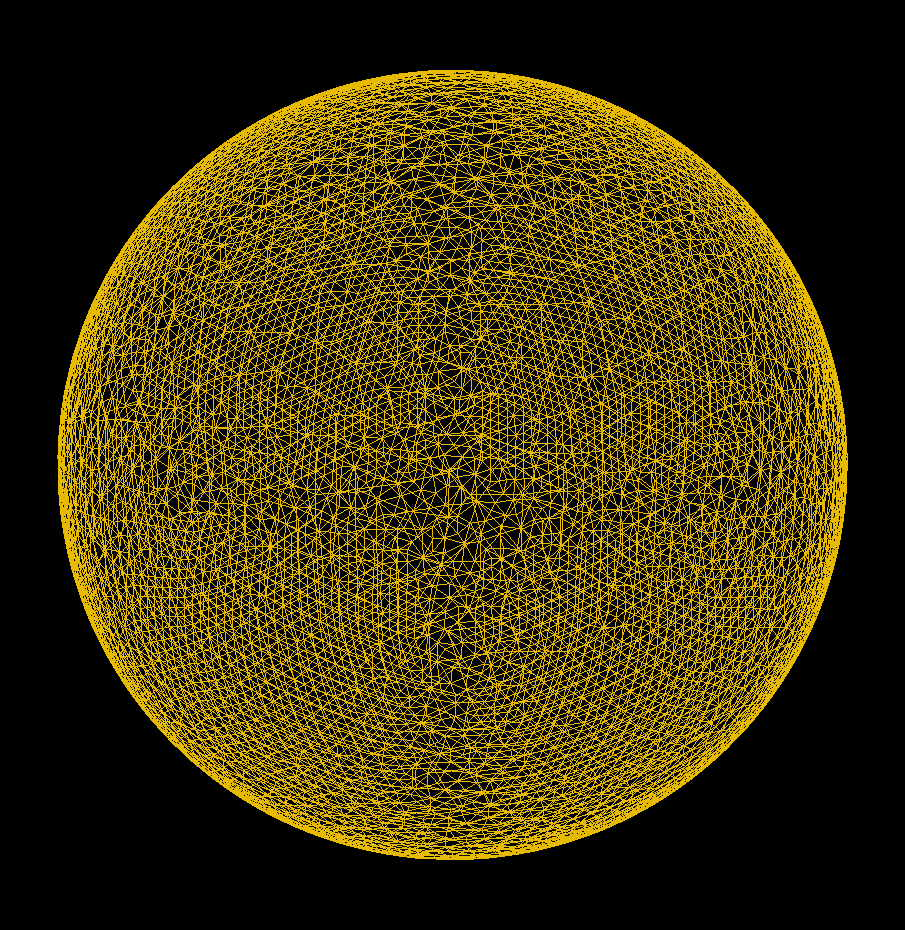
\includegraphics[width=0.3\linewidth]{a.png}
      }
  \hspace{0.5in} % 两图片之间的距离
  \subfigure[rocker,simplification ratio = 0.8]{
      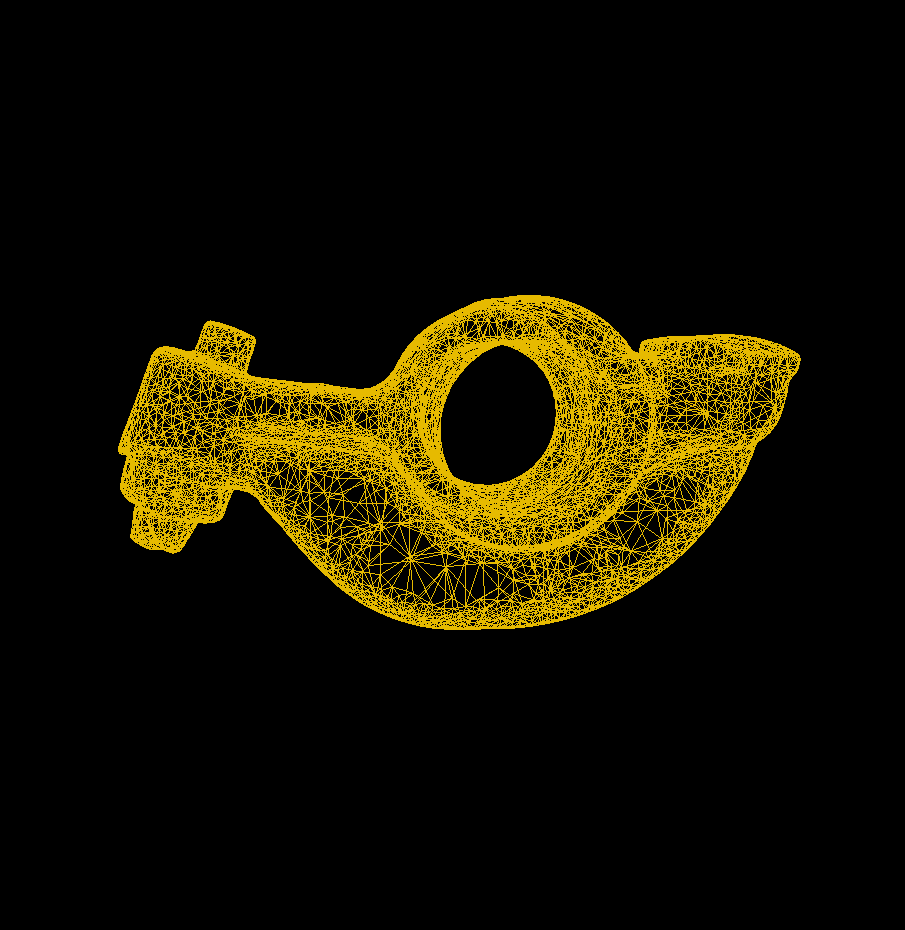
\includegraphics[width=0.3\linewidth]{simplification_1_rocker.png}
      }
  \hspace{0.5in} % 两图片之间的距离
  \subfigure[dinosaur,simplification ratio = 0.8]{
    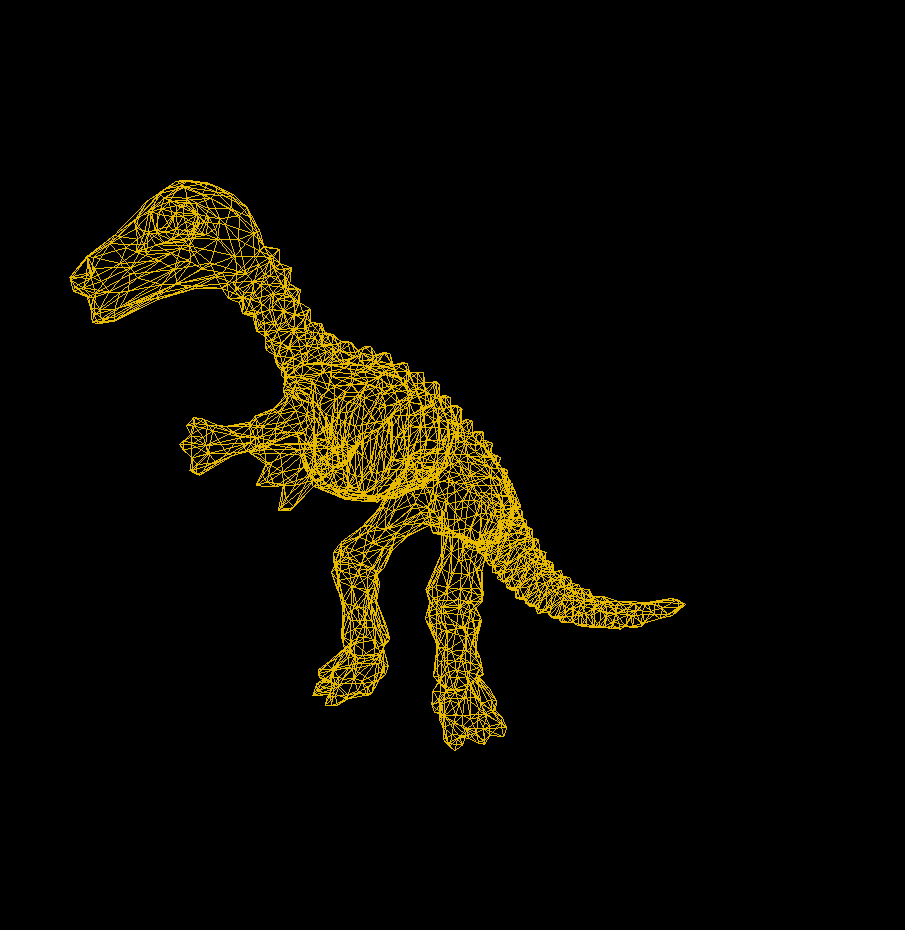
\includegraphics[width=0.3\linewidth]{simplification_1.png}
    }
  \hspace{0.5in} % 两图片之间的距离
  \subfigure[dinosaur,simplification ratio = 0.6]{
      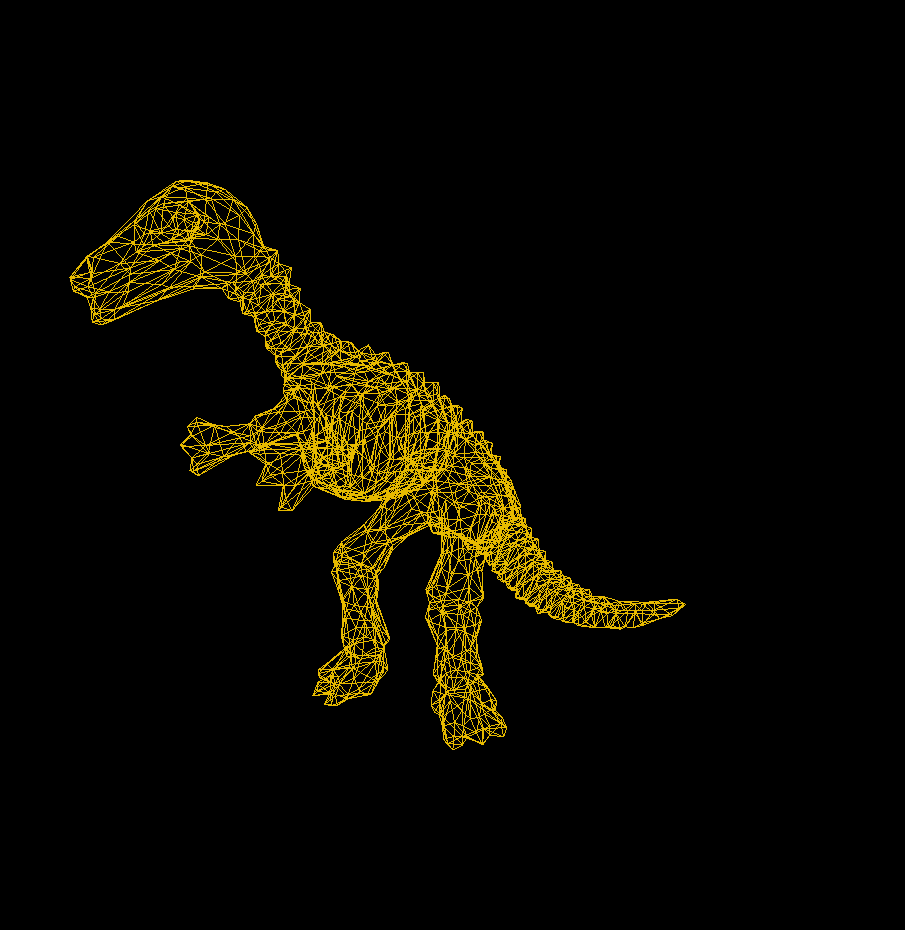
\includegraphics[width=0.3\linewidth]{simplification_2.png}
      }
  \hspace{0.5in} % 两图片之间的距离
  \subfigure[dinosaur,simplification ratio = 0.4]{
  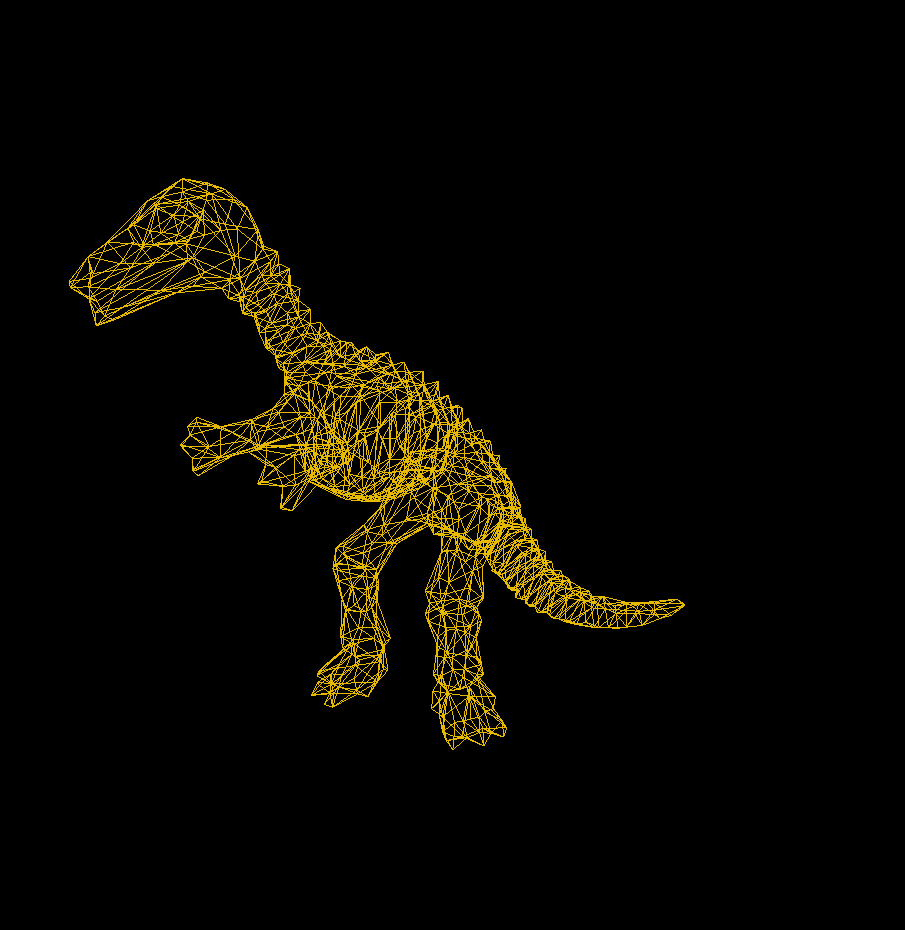
\includegraphics[width=0.3\linewidth]{simplification_3.png}
    }
    \hspace{0.5in}
  \subfigure[dinosaur,simplification ratio = 0.2]{
  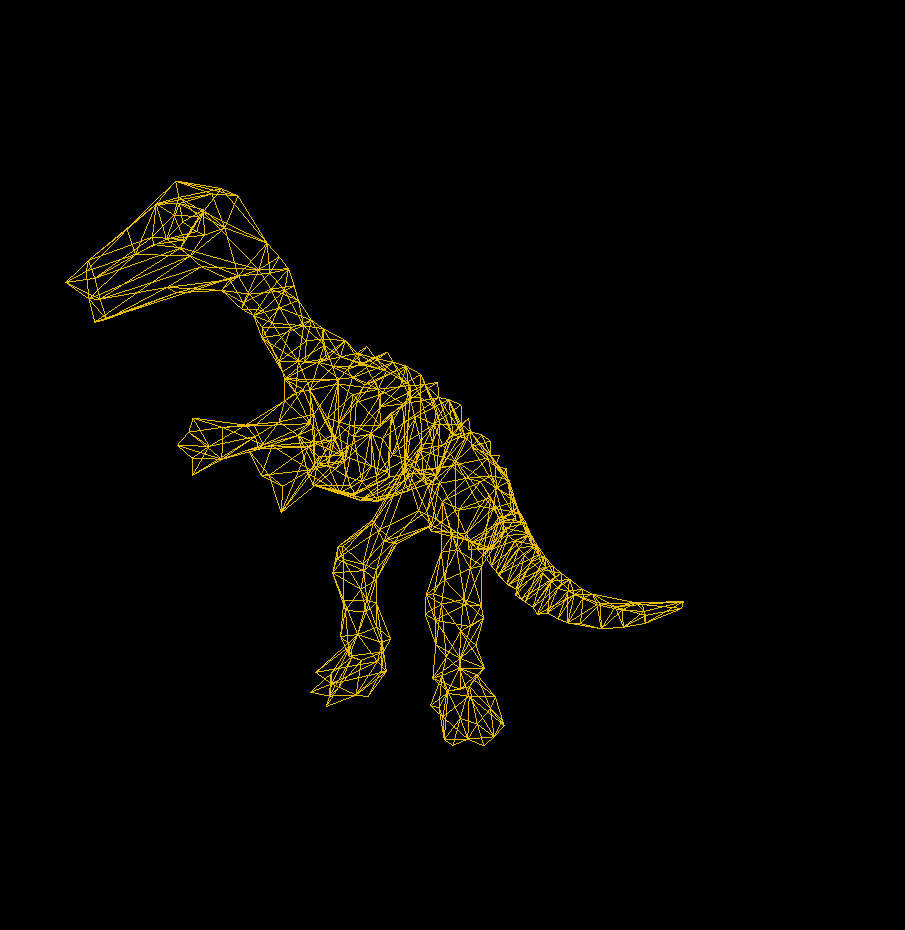
\includegraphics[width=0.3\linewidth]{simplification_4.png}
    }
  \caption{Mesh Simplification}
\end{figure}
\section{Mesh Smoothing}
算法大致流程:

\begin{enumerate}
    \item 对于每个顶点,计算邻居位置的加权平均
        $$v_i^*=\frac{\sum_{j\in N(i)}w_{ij} v_j}{\sum_{j\in N(i)} w_{ij}}$$
    \item 其中使用 Uniform Laplacian 时 $w_{ij}=1$ ;使用 Cotangent Laplacian 时 $w_{ij}=\cot \alpha_{ij} + \cot \beta_{ij}$.
            在计算$\cot \alpha_{ij}$和$\cot \beta_{ij}$时,先计算出两个角的余弦值。而经过尝试,直接用两个向量的点乘直接代替余弦值效果更好。
    \item 更新顶点:$v_i=(1-\lambda)v_i+\lambda v_i^*$
    \item 重复上述步骤直到达到迭代次数
\end{enumerate}

得到结果如图:
\begin{figure}[H]
    \centering
    \subfigure[Cotangent, numIteration=1,$\lambda$=0.7]{
        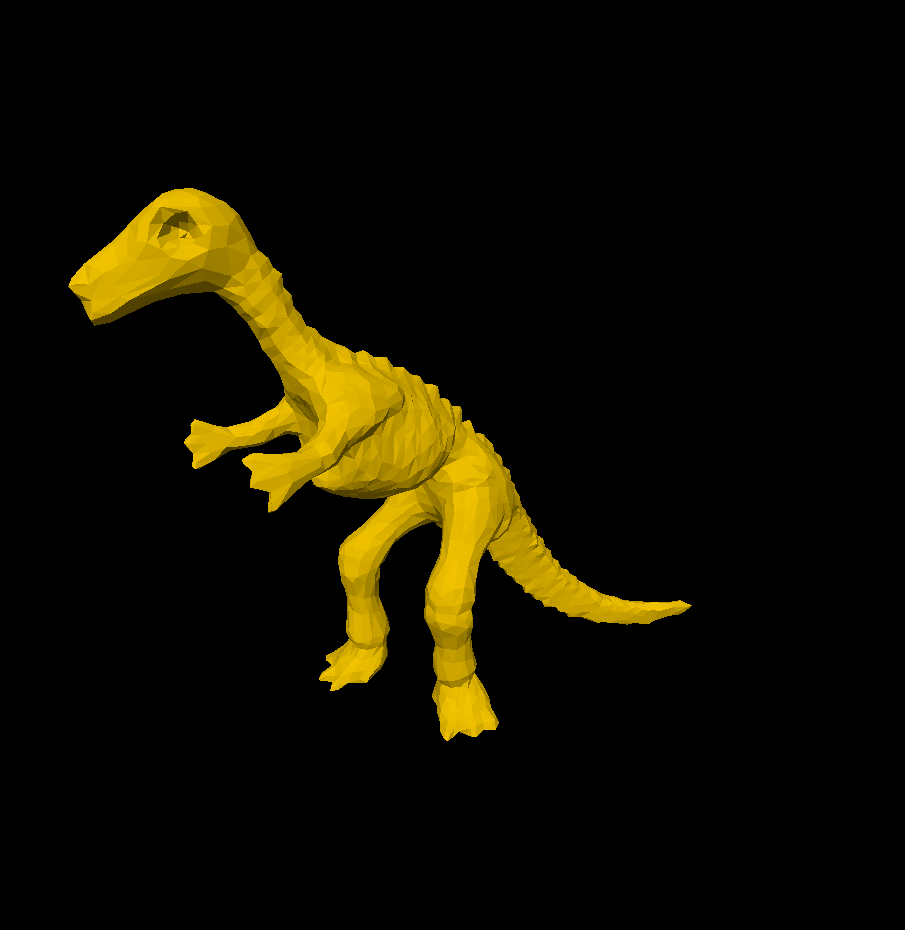
\includegraphics[width=0.3\linewidth]{cot_1_0.7.png}
        }
    \hspace{0.5in} % 两图片之间的距离
    \subfigure[Cotangent, numIteration=5,$\lambda$=0.7]{
      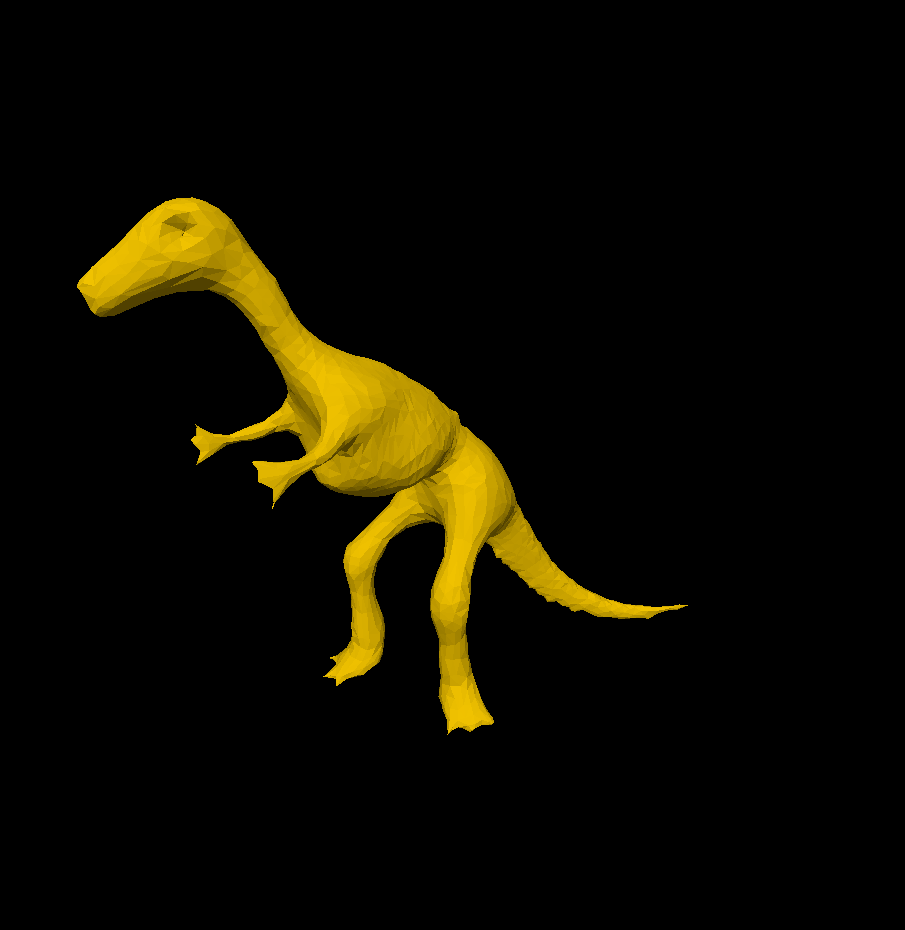
\includegraphics[width=0.3\linewidth]{cot_5_0.7.png}
      }
    \hspace{0.5in} % 两图片之间的距离
    \subfigure[Cotangent, numIteration=10,$\lambda$=0.7]{
        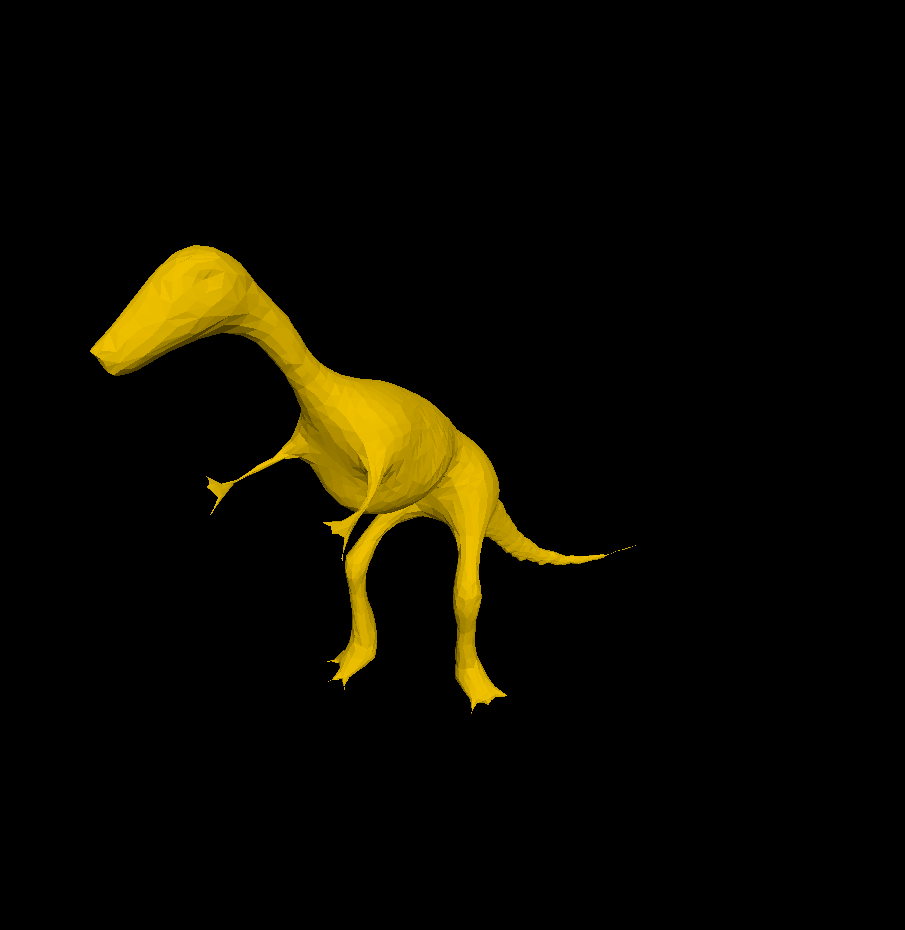
\includegraphics[width=0.3\linewidth]{cot_10_0.7.png}
        }
    \hspace{0.5in} % 两图片之间的距离
    \subfigure[Uniform, numIteration=1,$\lambda$=0.7]{
    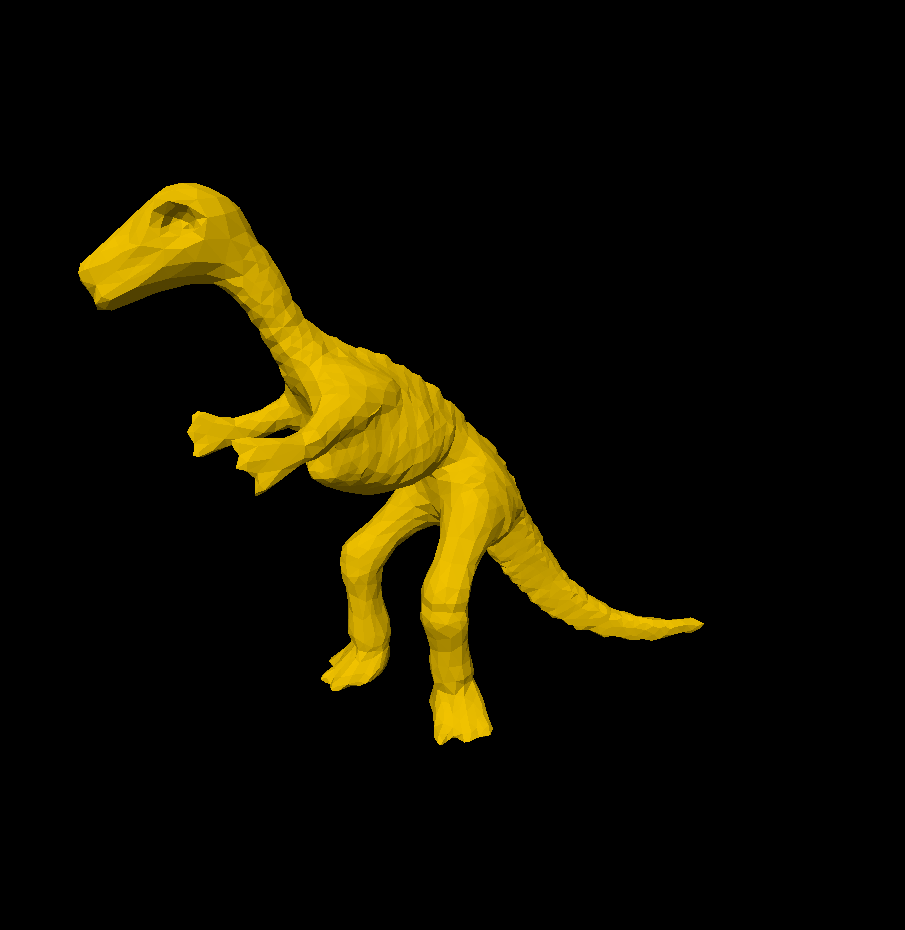
\includegraphics[width=0.3\linewidth]{uni_1_0.7.png}
      }
      \hspace{0.5in}
    \subfigure[Uniform, numIteration=5,$\lambda$=0.7]{
    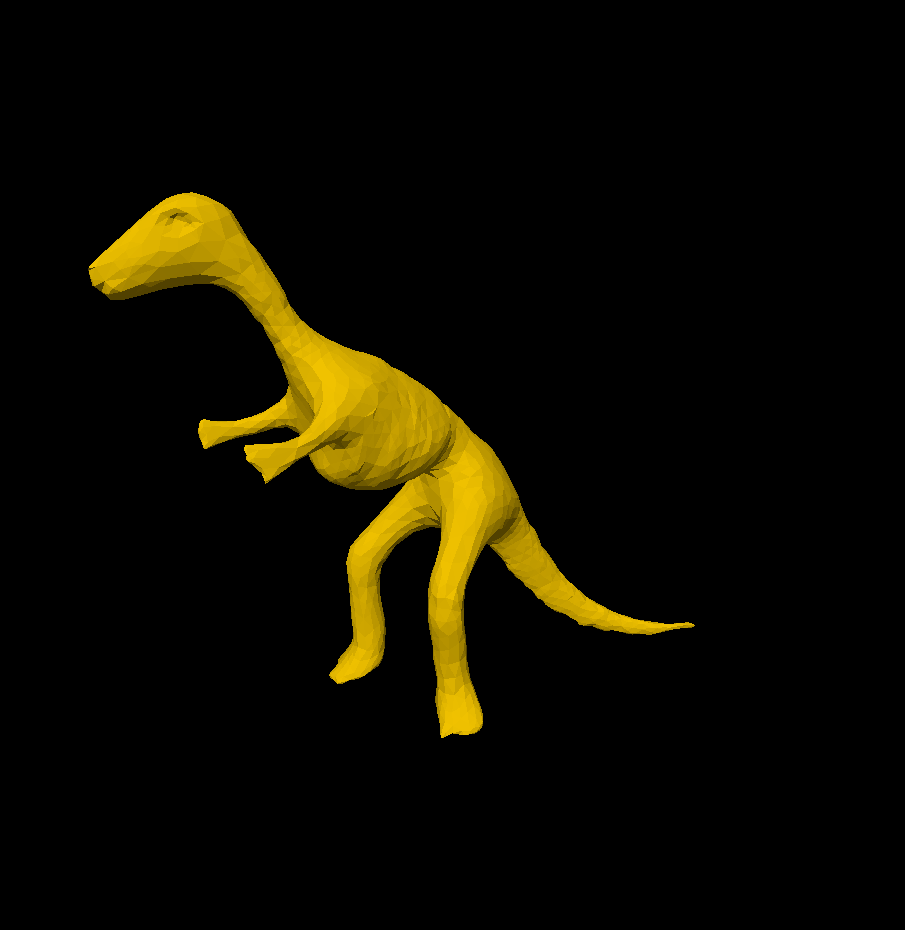
\includegraphics[width=0.3\linewidth]{uni_5_0.7.png}
      }
    \hspace{0.5in}
    \subfigure[Uniform, numIteration=10,$\lambda$=0.7]{
        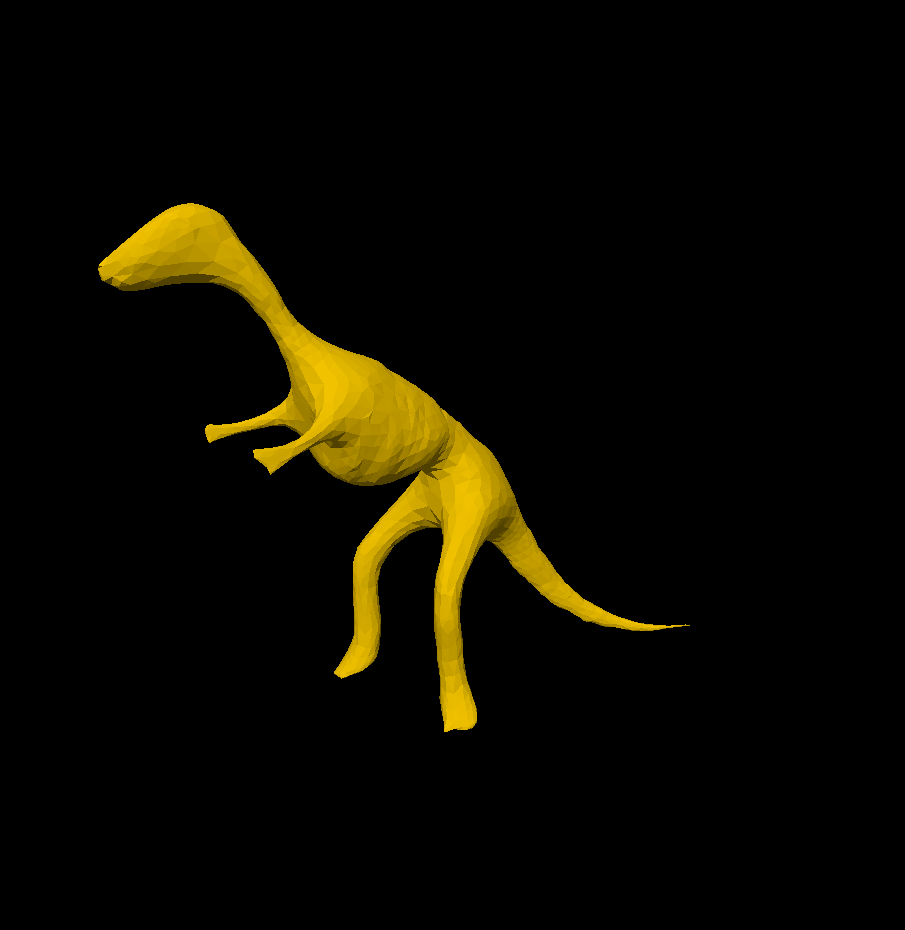
\includegraphics[width=0.3\linewidth]{uni_10_0.7.png}
      }
    \caption{Mesh Smoothing}
\end{figure}

可以看到使用Cotangent Laplacian得到的结果相比与使用Uniform Laplacian得到的结果更加尖锐,在爪子、脚趾处结构保留更好,但是手臂、腿明显更为退化。

\section{Marching Cubes}
算法大致流程:

依次对每一个小立方体执行以下步骤:
\begin{enumerate}
    \item 计算该立方体的$index$: 如果编号为$i$的顶点到隐式表面的有向距离小于等于0,则$index$的第$i$位为1,否则为0.
    \item 如果$index = 0 or 255$,说明这个立方体与隐式表面没有交点,前进到下一个立方体。
    \item 否则找到$c_EdgeOrdsTable[Index]$数组,里面的数字按顺序每三个一组,为隐式表面与立方体相交得到的三角形顶点所在的边,
            按照线性插值公式$P =P_0 + \frac{-sdf(P_0)}{sdf(P_1) - sdf(P_0)} \times (P_1 - P_0)$得到该顶点的位置.
    \item 若该点不在Positions数组中,则插入.更新Indices数组,并前进到下一个立方体.
\end{enumerate}

得到结果如图:
\begin{figure}[H]
    \centering
    \subfigure[sphere,n = 10]{
        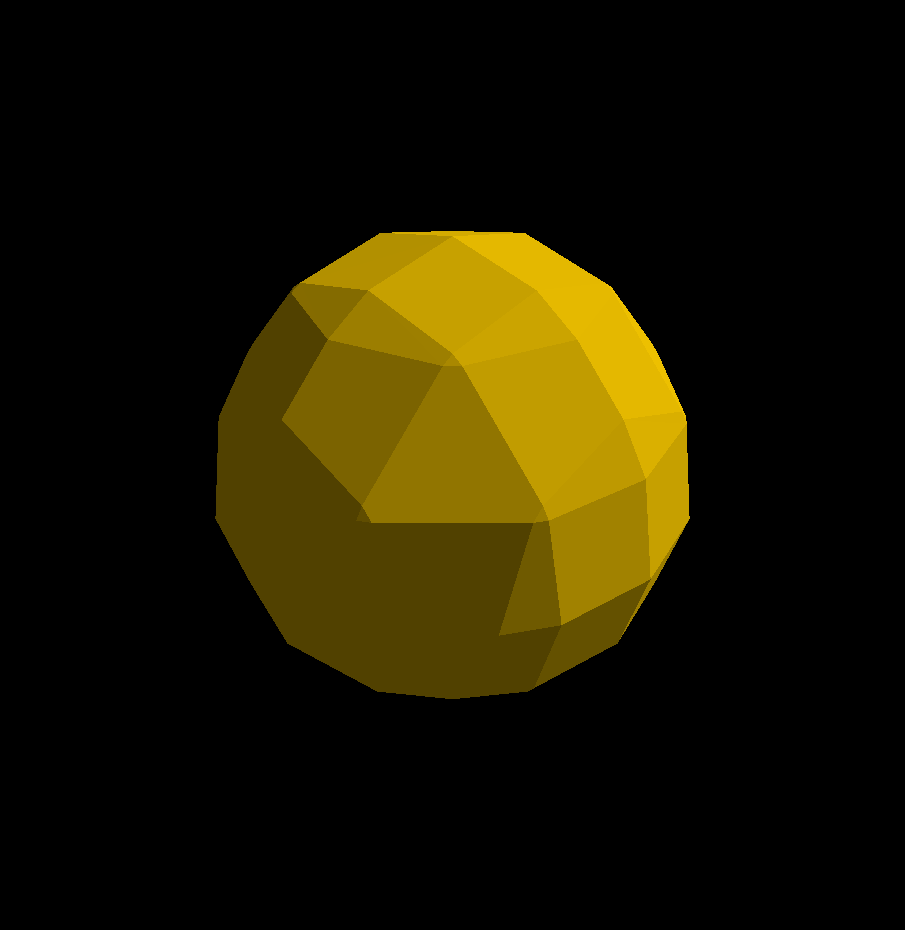
\includegraphics[width=0.3\linewidth]{marching_sphere_10.png}
        }
    \hspace{0.5in} % 两图片之间的距离
    \subfigure[sphere,n = 60]{
      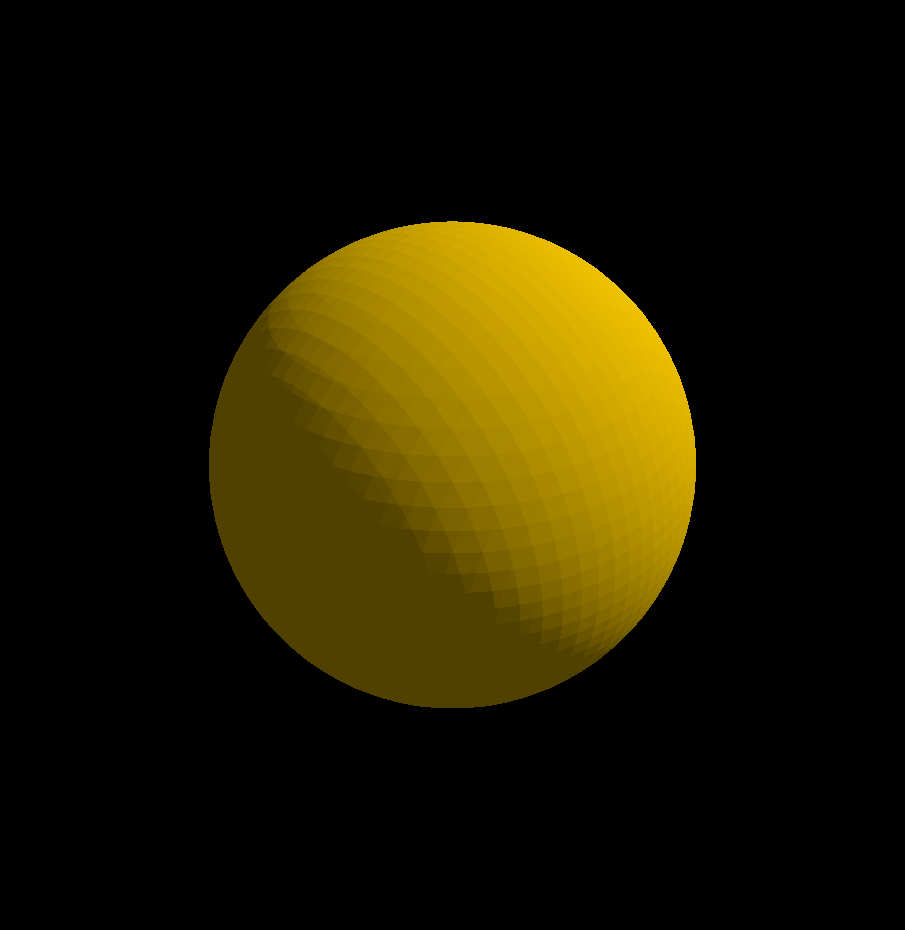
\includegraphics[width=0.3\linewidth]{marching_sphere_60.png}
      }
    \hspace{0.5in} % 两图片之间的距离
    \subfigure[sphere,n = 100]{
        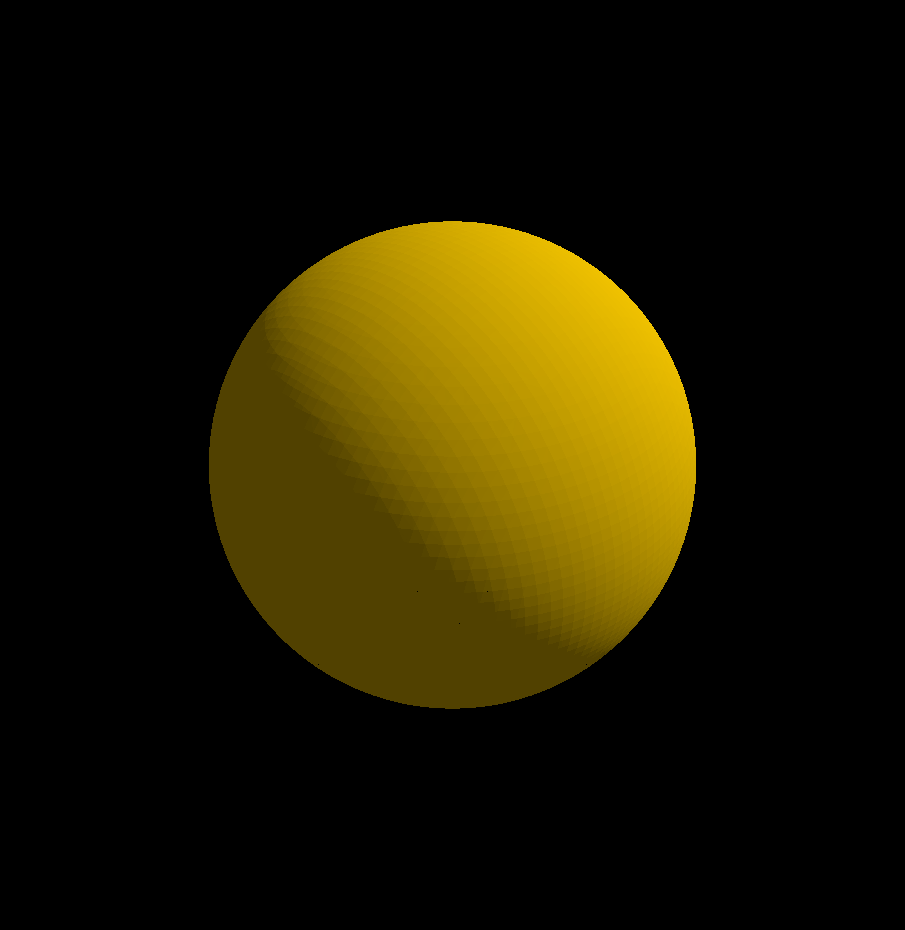
\includegraphics[width=0.3\linewidth]{marching_sphere_100.png}
        }
    \hspace{0.5in} % 两图片之间的距离
    \subfigure[torus,n = 10]{
    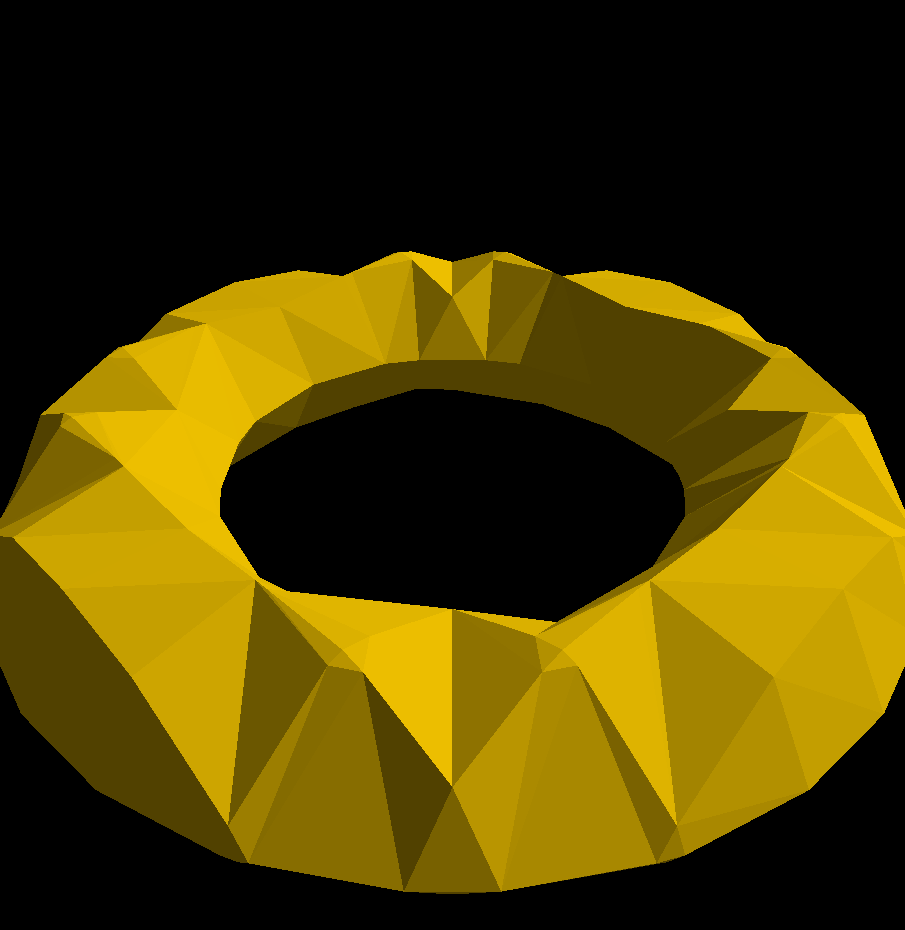
\includegraphics[width=0.3\linewidth]{marching_torus_10.png}
      }
      \hspace{0.5in}
    \subfigure[torus,n = 60]{
    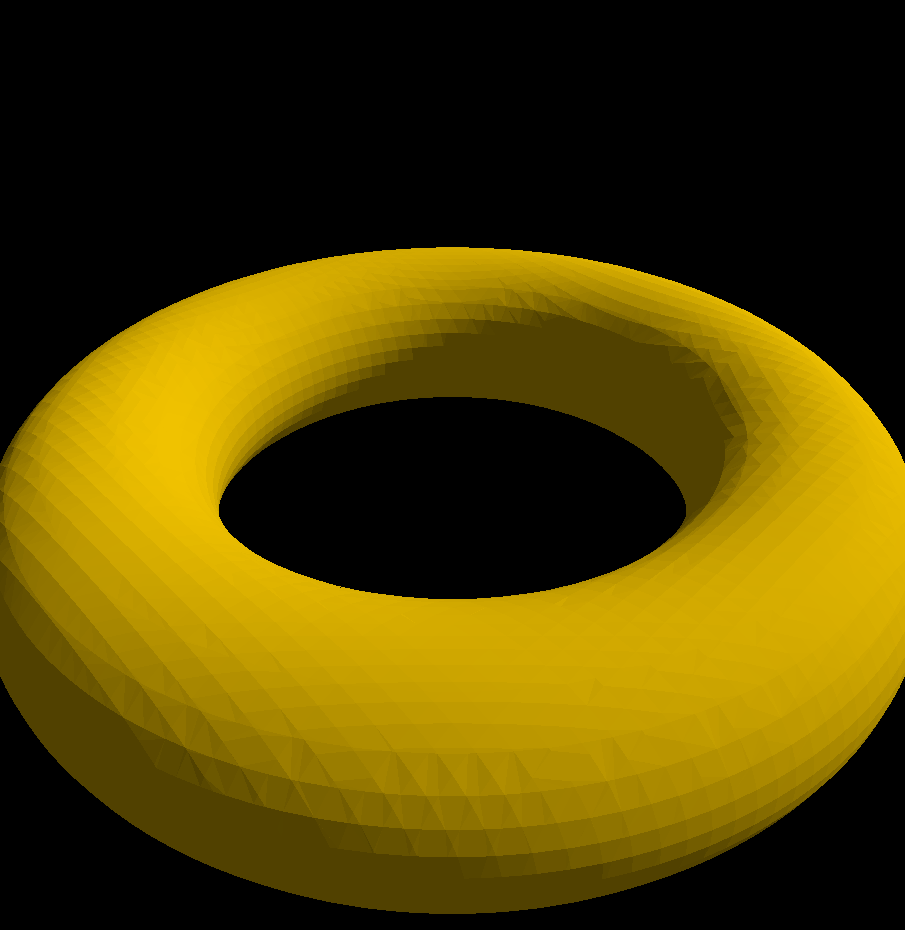
\includegraphics[width=0.3\linewidth]{marching_torus_60.png}
      }
    \hspace{0.5in}
    \subfigure[torus,n = 100]{
        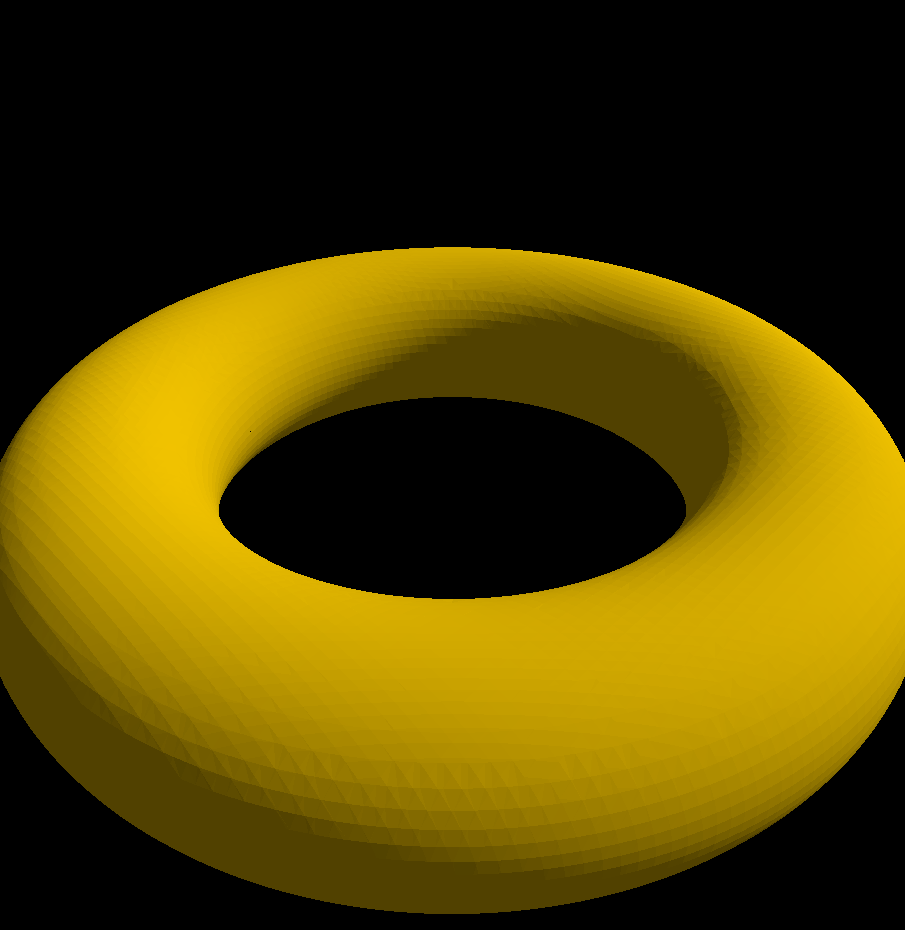
\includegraphics[width=0.3\linewidth]{marching_torus_100.png}
      }
    \caption{Marching Cubes}
\end{figure}

\end{document}